
\documentclass[10pt, conference]{IEEEtran}


% *** CITATION PACKAGES ***
%
%\usepackage{natbib}
%\usepackage{cite}
% cite.sty was written by Donald Arseneau
% V1.6 and later of IEEEtran pre-defines the format of the cite.sty package
%$ \cite{} output to follow that of IEEE. Loading the cite package will
% result in citation numbers being automatically sorted and properly
% "compressed/ranged". e.g., [1], [9], [2], [7], [5], [6] without using
% cite.sty will become [1], [2], [5]--[7], [9] using cite.sty. cite.sty's
% \cite will automatically add leading space, if needed. Use cite.sty's
% noadjust option (cite.sty V3.8 and later) if you want to turn this off.
% cite.sty is already installed on most LaTeX systems. Be sure and use
% version 4.0 (2003-05-27) and later if using hyperref.sty. cite.sty does
% not currently provide for hyperlinked citations.
% The latest version can be obtained at:
% http://www.ctan.org/tex-archive/macros/latex/contrib/cite/
% The documentation is contained in the cite.sty file itself.




% *** GRAPHICS RELATED PACKAGES ***
%
\ifCLASSINFOpdf
   \usepackage[pdftex]{graphicx}
  % declare the path(s) where your graphic files are
   \graphicspath{{../pdf/}{../jpeg/}}
  % and their extensions so you won't have to specify these with
  % every instance of \includegraphics
   \DeclareGraphicsExtensions{.pdf,.jpeg,.png}
\else
  % or other class option (dvipsone, dvipdf, if not using dvips). graphicx
  % will default to the driver specified in the system graphics.cfg if no
  % driver is specified.
  % \usepackage[dvips]{graphicx}
  % declare the path(s) where your graphic files are
  % \graphicspath{{../eps/}}
  % and their extensions so you won't have to specify these with
  % every instance of \includegraphics
  % \DeclareGraphicsExtensions{.eps}
\fi
% graphicx was written by David Carlisle and Sebastian Rahtz. It is
% required if you want graphics, photos, etc. graphicx.sty is already
% installed on most LaTeX systems. The latest version and documentation can
% be obtained at: 
% http://www.ctan.org/tex-archive/macros/latex/required/graphics/
% Another good source of documentation is "Using Imported Graphics in
% LaTeX2e" by Keith Reckdahl which can be found as epslatex.ps or
% epslatex.pdf at: http://www.ctan.org/tex-archive/info/
%
% latex, and pdflatex in dvi mode, support graphics in encapsulated
% postscript (.eps) format. pdflatex in pdf mode supports graphics
% in .pdf, .jpeg, .png and .mps (metapost) formats. Users should ensure
% that all non-photo figures use a vector format (.eps, .pdf, .mps) and
% not a bitmapped formats (.jpeg, .png). IEEE frowns on bitmapped formats
% which can result in "jaggedy"/blurry rendering of lines and letters as
% well as large increases in file sizes.
%
% You can find documentation about the pdfTeX application at:
% http://www.tug.org/applications/pdftex


\let\labelindent\relax
\usepackage{paralist}

\usepackage{enumitem}
\newlist{RQ}{enumerate}{1}
\setlist[RQ]{label=RQ\arabic*:,leftmargin=3\parindent}

\usepackage[colorinlistoftodos]{todonotes}



% correct bad hyphenation here
\hyphenation{op-tical net-works semi-conduc-tor}


\begin{document}
%
% paper title
% can use linebreaks \\ within to get better formatting as desired
\title{Characterizing the development of a cross-platform library: a case study of Allegro}
% by mining commit logs
% Mining and Characterizing Cross-Platform libraries


% author names and affiliations
% use a multiple column layout for up to two different
% affiliations

\author{\IEEEauthorblockN{Authors Name/s per 1st Affiliation (Author)}
\IEEEauthorblockA{line 1 (of Affiliation): dept. name of organization\\
line 2: name of organization, acronyms acceptable\\
line 3: City, Country\\
line 4: Email: name@xyz.com}
\and
\IEEEauthorblockN{Authors Name/s per 2nd Affiliation (Author)}
\IEEEauthorblockA{line 1 (of Affiliation): dept. name of organization\\
line 2: name of organization, acronyms acceptable\\
line 3: City, Country\\
line 4: Email: name@xyz.com}
}

% conference papers do not typically use \thanks and this command
% is locked out in conference mode. If really needed, such as for
% the acknowledgment of grants, issue a \IEEEoverridecommandlockouts
% after \documentclass

% for over three affiliations, or if they all won't fit within the width
% of the page, use this alternative format:
% 
%\author{\IEEEauthorblockN{Michael Shell\IEEEauthorrefmark{1},
%Homer Simpson\IEEEauthorrefmark{2},
%James Kirk\IEEEauthorrefmark{3}, 
%Montgomery Scott\IEEEauthorrefmark{3} and
%Eldon Tyrell\IEEEauthorrefmark{4}}
%\IEEEauthorblockA{\IEEEauthorrefmark{1}School of Electrical and Computer Engineering\\
%Georgia Institute of Technology,
%Atlanta, Georgia 30332--0250\\ Email: see http://www.michaelshell.org/contact.html}
%\IEEEauthorblockA{\IEEEauthorrefmark{2}Twentieth Century Fox, Springfield, USA\\
%Email: homer@thesimpsons.com}
%\IEEEauthorblockA{\IEEEauthorrefmark{3}Starfleet Academy, San Francisco, California 96678-2391\\
%Telephone: (800) 555--1212, Fax: (888) 555--1212}
%\IEEEauthorblockA{\IEEEauthorrefmark{4}Tyrell Inc., 123 Replicant Street, Los Angeles, California 90210--4321}}





% use for special paper notices
%\IEEEspecialpapernotice{(Invited Paper)}




% make the title area
\maketitle

%%%%%%%%%%%%%%%%%%%%%%%%%%%%%%%%%%%%%%%%
%%%%%%%%%%%%%%%%%%%%%%%%%%%%%%%%%%%%%%%%%
%%%%%%%%%%%%%%%%%%%%%%%%%%%%%%%%%%%%%%%%%
\begin{abstract}
As new operating systems and hardware devices emerge and become popular, developers demand libraries to help them build cross-platform applications. Nevertheless, there is a lack of knowledge about the development process of such libraries. With the goal of characterizing the development of cross-platform libraries, we analyzed the commit log of Allegro, a successful cross-platform multimedia library written in C. We found that 52.4\% of the developers contribute to two or more platforms. Moreover, we identified that core developers contribute to significantly more platforms and device types than peripheral developers. As future work, we plan to replicate this study in order to validate our conclusions with other cross-platforms libraries.

\end{abstract}

\begin{IEEEkeywords}
cross-platform development; software libraries; version control system.

\end{IEEEkeywords}


% For peer review papers, you can put extra information on the cover
% page as needed:
% \ifCLASSOPTIONpeerreview
% \begin{center} \bfseries EDICS Category: 3-BBND \end{center}
% \fi
%
% For peerreview papers, this IEEEtran command inserts a page break and
% creates the second title. It will be ignored for other modes.
\IEEEpeerreviewmaketitle

% Challenges of running / maintaining a cross-platform library project -- specialization of developers
  % We conjecture that successful projects are led by developers who master multiple platforms
  % Some platforms have more isolated communities, making it difficult to find developers for those platforms that also develop for other platforms
  % If you know platform X, you're likely to know platform Y, making it easier to find people who know both X and Y
% platform is more independent => the code is very different from other platforms


%%%%%%%%%%%%%%%%%%%%%%%%%%%%%%%%%%%%%%
%%%%%%%%%%%%%%%%%%%%%%%%%%%%%%%%%%%%%%
%%%%%%%%%%%%%%%%%%%%%%%%%%%%%%%%%%%%%%
\section{Introduction}
% no \IEEEPARstart

%\todo[inline]{Este paragrafo deveria estar no inicio.}

Software developers are constantly faced with challenge of making their software run on multiple platforms so it can reach a larger user base. To facilitate this task, developers can rely on cross-platform libraries, which encapsulate platform-specific code for multiple platforms.

%Software users are segmented by the many platforms that exist currently, and new platforms become popular from time to time to support new devices and usage scenarios. Software developers, on the other end, are constantly faced with challenge of making their software run on the most widespread platforms.

%Cross-platform libraries are in demand by developers because of the scenario with many platforms. Moreover, new platforms can start a trend and claim support by popular demand, making developers upgrading the software. 

%\todo[inline]{Continuo achando que essa primeira frase esta estranha. Veja os comentarios em https://goo.gl/PD2Mei}
Cross-platform libraries allow developers to write cross-platform applications without knowing all the technical aspects of the target platforms. Each platform can have a unique approach to implement a functionality or communicate with a hardware device. Hence, to build a cross-platform software, the developer would need to write some platform-specific code~\cite{bishop2006,backblaze2008}. It is considered a good programing practice to use as much as possible platform-independent code~\cite{bishop2006,backblaze2008}. 



%Companies want to make their products available for as many platforms as possible but developing a cross-platform application can be costly and some companies choose to limit the number of platforms in the initial version and port it later to other platforms~\cite{Fahy2012}. Porting it later can make it much more expensive as the developer will have to review what have been done first~\cite{Fahy2012,bishop2006}. 

Despite the importance of cross-platform libraries, little is known about how they are developed. The development of such libraries pose unique challenges. Cross-platform libraries may break in some point due to  platform changes, requiring their developers to evolve the library code~\cite{bishop2006}. Also,  developers need specific knowledge and tools to develop for every single platform.

The development of cross-platform libraries requires platform's technical expertises. Therefore, it is expected to be performed by a team of developers with experience in at least one platform, but the ideal case is to have developers with experience in all target platforms. Some maintenance tasks might require changes in the code of many platforms, requiring a coordination among the specialized developers of all platforms involved or an intervention of a generalist developer, who support all platforms involved. 

The success of an open source project depends on the contribution of both core developers, who actively contribute to the project, and peripheral developers, who contribute sporadically. For open source cross-platform libraries, we have no information about the distribution of platforms among core and peripheral developers in successful projects.

%Cross-platform libraries are sensitive to changes in the platforms they support, 
%because it can make parts of the system to fail. Analogously,  a hardware change can also affect some parts of the system~\cite{bishop2006}. A platform change is critical for cross-platform libraries and cannot be ignored or postponed.   
%to handle with the different hardware architecture and implementations of file system, graphic user interface (GUI), audio system, security cite{bishop2006,backblaze2008}.
%Compiled languages require compiling for each platform it supports. Libraries such as Simple DirectMedia Layer (SDL) and Allegro have implementations for multiple platforms and allow developers to code for the library used instead of the target platforms.     

In order to better understand the development process of open source cross-platform libraries, we conducted a preliminary case study of Allegro, a multimedia library for Windows, Linux, macOS\footnote{Previously known as Mac OS X.}, Android, and iPhone. By analyzing its commit log, we aimed to answer the following research questions:

%In this paper we are interested to know some characteristics about cross-platform library projects. We selected Allegro to work on and we used the information available in the repository to answer the following research questions:

\begin{RQ}
% \item  Which platform is more independent in terms of being modified alone during maintenance tasks? \todo[inline]{Which platforms tend to change when there is a change in platform-independente code?}
\item Do core developers tend to contribute with more platforms than peripheral developers?
\item Is there a clear separation between mobile and desktop developers?
\item  Which platforms are more related together considering the set of platforms a developer work with? 
\end{RQ}



%The remainder of this paper is organized as follows: Section X…. 

\section{Background}

To achieve the goal of building a cross-platform application in the scenario of many device types and platforms, developers should consider three fundamental requirements~\cite{Levin2014}: an application should be consistent, continuous and complementary. Consistent design means that the core functionalities and structure are kept across platforms. Continuous design is when a user can start an activity in one platform and finish it in some other platform. Complementary design is that devices complement one another with a relevant functionality that only a specific device can do.   


%\todo[inline]{citation required in "raises overall quality of the code"}

Building cross-platform raises the overall quality of code and the range of users who can take advantage of the software~\cite{backblaze2008}. A software engineer of Backblaze reported some guidelines for writing cross-platform code in C and C++ \cite{backblaze2008}, we selected 4 rules strongly related to our research:

%\todo[inline]{Select only some rules}
\begin{enumerate}
\item Simultaneously development - Think about cross-platform from the very beginning of a project.  
%\item XML for GUI - Factor out the GUI into non reusable code and then develop a cross-platform library for the underlying logic.
%\item Use standard C types, not platform-specific types.
%\item Use only built in \#ifdef compiler flags, do not invent your own.
\item Develop a simple set of reusable, cross-platform base libraries to hide platform-specific code
%\item Use Unicode, specifically UTF-8, for all APIs.
\item Don't use third-party application frameworks or runtime environments. 
%\item Build the raw source directly on all platforms.
\item Require all programmers to compile on all platforms.
%\item Fire the lazy, incompetent, or bad attitude programmers who can’t follow these rules.
\end{enumerate}

%Conversely to the guidelines 2 and 3, companies can take advantage of cross-platform libraries reducing the development time, but some companies reject this option thinking those libraries are not suitable for them~\cite{Fahy2012}.

At Avaya, since it is hard to find qualified developers with experience in many platforms, Avaya's development team  was divided in pure desktop and Windows team and pure mobile team. The division of the team hid the low experience of developers with the development of cross-platform software, but it hinders fixing bugs in all supported platforms and create redundant development effort in some cases \cite{Duc2014}.  %\todo{Rever}

%Avaya's projects use fork to outsource development team. As 


%\todo[inline]{Podia aproveitar e fazer um gancho, dizendo que neste trabalho voce vai caracterizar um projeto open source bem-sucedido quando aa atribuicao de plataformas a desenvolvedores.}


%%%%%%%%%%%%%%%%%%%%%%%%%%%%%%%%%%%%%%
%%%%%%%%%%%%%%%%%%%%%%%%%%%%%%%%%%%%%%
%%%%%%%%%%%%%%%%%%%%%%%%%%%%%%%%%%%%%%
\section{Methodology}
\label{methodology}

In order to establish relations among platforms and be aware of the developer team profile of cross-platform library projects, we selected Allegro library to conduct the study. Table~\ref{allegrogeneral} shows a summary of Allegro's general characteristics.  

\begin{table}[h]
%% increase table row spacing, adjust to taste
\renewcommand{\arraystretch}{1.3}
\caption{Allegro's general characteristics}
\label{allegrogeneral}
\centering

\begin{tabular}{|c|c|}
\hline
Type & Multimedia and Games SDK \\
\hline
First release & 1990 \\
\hline
Language & C \\
\hline
Licence & zlib \\
\hline
Platforms & Windows, Linux, macOS, iPhone, Android \\
\hline
\end{tabular}
\end{table}

We extracted the commits related to modifications from Allegro's repository. The Table \ref{allegroinfo} shows the release selected, some size metrics, the analysis period  and the quantity of commits extracted from Allegro's repository.  


%\todo[inline]{Add number of developers}

\begin{table}[h]
\renewcommand{\arraystretch}{1.3}
\caption{Allegro’s development informationm}
\label{allegroinfo}
\centering
\begin{tabular}{|c|c|c|}
\hline
Release & 5.2.1.1\\
\hline
LOC & 79.004 \\
\hline
Modules & 144\\
\hline
Packages & 13\\
\hline
Functions & 2.358\\
\hline
Developers & 21 \\
\hline
Commits & 1.143  \\
\hline
Period & 01/12/2011 - 01/12/2016   \\
\hline
\end{tabular}
\end{table}

Allegro's first release supported Windows, macOS, and Linux. Then in August 2009 they started supporting iPhone and in December 2011 they started supporting Android. As our intention was to study all five platforms, we extracted the commits from 1st December 2011 until 1st December 2016, totalizing 1143 commits.  

%Despite 
Although Allegro supports officially five platforms, as shown in Table~\ref{allegrogeneral}, we considered Unix as a sixth platform as it is developed in a package separated from Linux, and many other packages are logically coupled with Unix package. Figure~\ref{diagrama} shows a UML diagram of logical coupling among packages of Allegro. 

\begin{figure}[h]
\centering
\textbf{}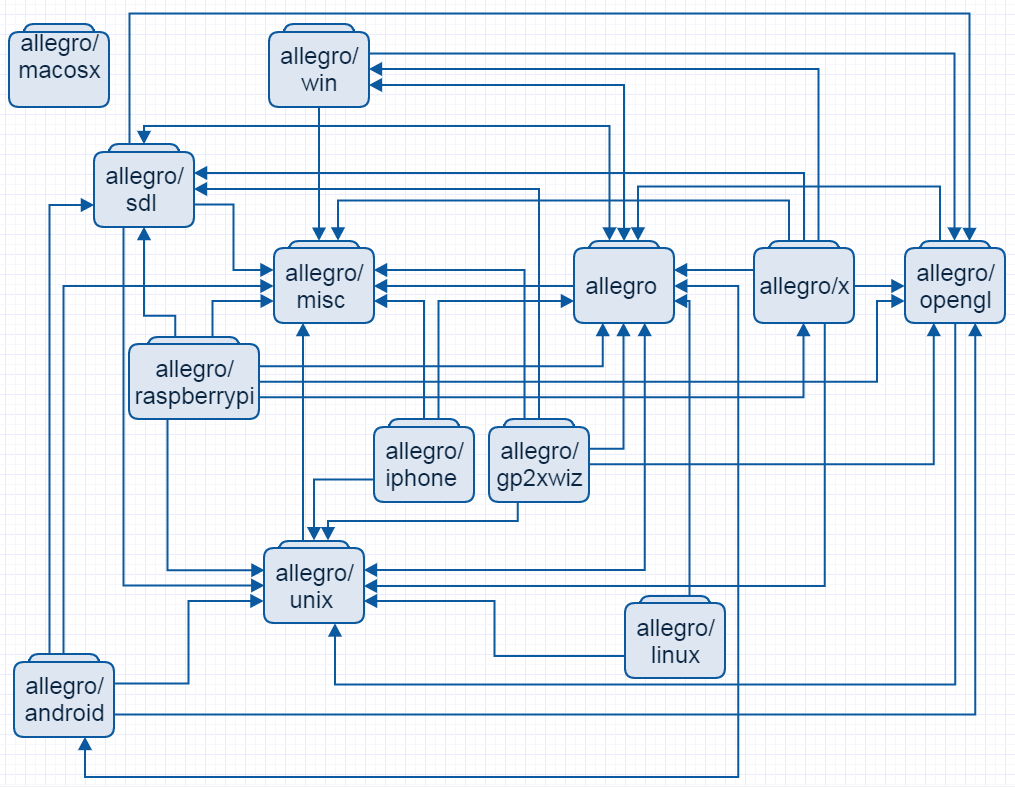
\includegraphics[width=2.5in]{diagrama}
\caption{UML diagram of logical coupling among packages}
\label{diagrama}
\end{figure} 

%For the data mining and quantitative analysis we used the R, programming language and software environment for statistical computing and graphics. 
The study was designed as a three-part method, as illustrated in Figure~\ref{metodologia}: 

\begin{itemize}
\item Commit log extraction: Allegro uses Git, an open version control repository (VCS), and its commit log was obtained from Allegro's public repository.
\item Data processing: we identified the platforms modified by each commit and each developer, and then filtered and grouped the data to enable its analysis.
%The R was used to extract information about the platforms and developer team from Allegro's commit log. 
\item Quantitative analysis: %The analysis were also made in the R. 
For each research question a different analysis was required, as will be further explained in sections \ref{met_analysis1}, \ref{met_analysis2} and \ref{met_analysis3}.
\end{itemize}

\begin{figure}[h]
\centering
\textbf{}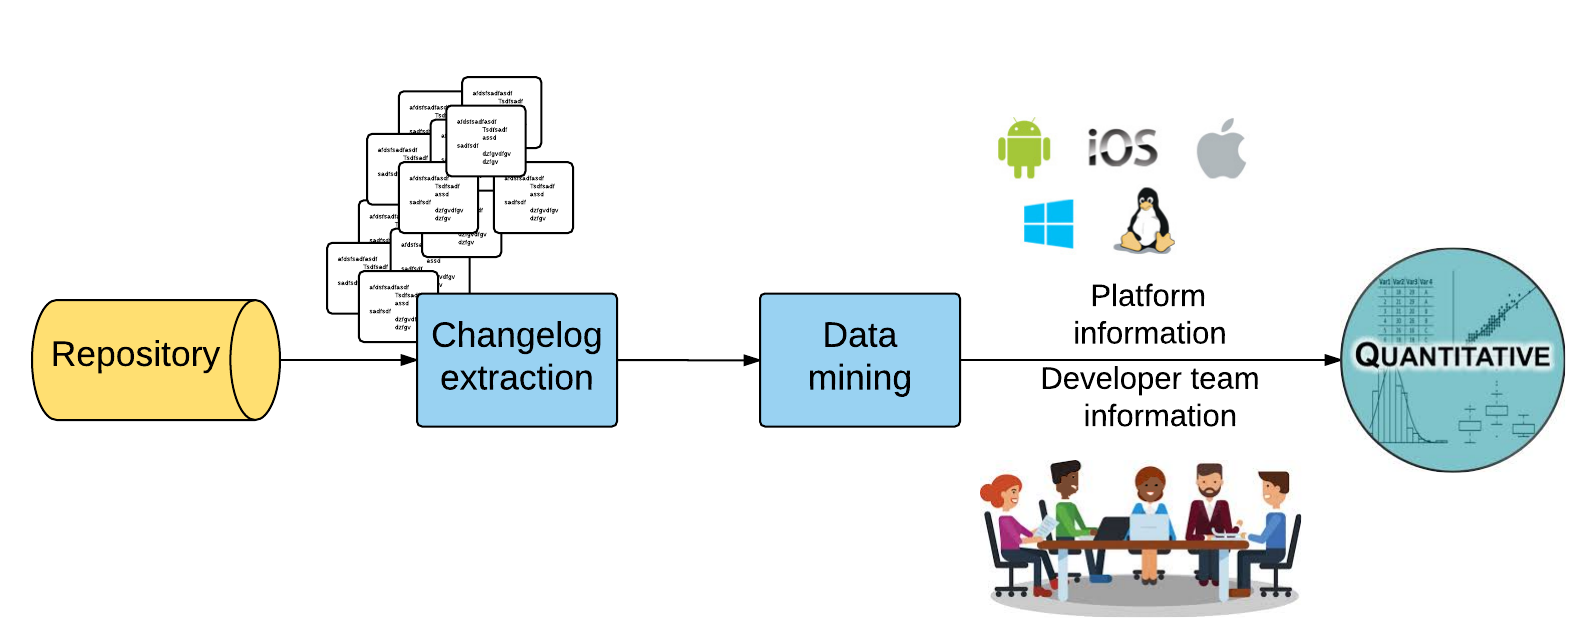
\includegraphics[width=3in]{metodologia}
\caption{Study fluxogram}
\label{metodologia}
\end{figure}

Allegro's platform-specific source code files are organized in packages (directories) according to the platform, as shown in Figure~\ref{diagrama}. Thus, to identify the platforms a developer works with, we listed all platform-specific code the developer has touched in the commits. We considered that a developer supports a certain platform if the developer has made at least one modification to a file inside the platform's package. 






%%%%%%%%%%%%%%%%%%%%%%%%%%%%%%%
\subsection{Analysis: Do core developers tend to contribute with more platforms than peripheral developers?}
\label{met_analysis1}

In order to determine whether core developers tend to contribute with more platforms than peripheral developers, we classified each developer as core or peripheral and counted the number of platforms each developer works with. 

The division was made by splitting the developer team by classifying the top 20\% committers as the core group and the remaining as the peripheral group~\cite{Robles2009}. Using this approach, the core group was responsible for 97.7\% of the total number of commits.

 

%%%%%%%%%%%%%%%%%%%%%%%%%%%%%%%%%
\subsection{Analysis: Is there a clear separation between mobile and desktop developers?}
\label{met_analysis2}

%\todo[inline]{Essa explicacao abaixo nao ficou clara. Para cada desenvolvedor, voce contou os commits para plataformas mobile e para plataformas desktop. Do jeito que esta explicado, parece que voce pegou todos os commits e dividiu em mobile e desktop, sem considerar a divisao por desenvolvedor.}


We listed all developers and we verified in the commit log the platforms the developers support. Then we grouped the platforms according to the device type: mobile (Android and iPhone) and desktop (Linux, Unix, Windows and macOS). %Therefore all the analysis were made considering  in mobile group and Linux, Unix, Windows and macOS in desktop group.  



%%%%%%%%%%%%%%%%%%%%%%%%%%%%%%%%%%%%%%
\subsection{Analysis: Which platforms are more related together considering the set of platforms a developer work with? }
\label{met_analysis3}

To determine which platforms are more interrelated considering the set of platforms a developer work with, we organized the data by developer and listed all platforms the developer works with and then we applied the Apriori algorithm for mining frequent set of platforms.The Apriori algorithm is a widely used association analysis algorithm. 

The association analysis is useful for finding interesting relationships in data  sets. The relations can be represented as association rules or set of frequent items \cite{Tan2005}. Considering the Table \ref{examplerule} as a example, the rule \{Diapers\} $\Rightarrow$ \{Beer\} suggests that the sale of diapers is strongly related to the sale of beer because many people who buy diapers also buy beer \cite{Tan2005}.   
\begin{table}[h]
\renewcommand{\arraystretch}{1.3}
\caption{Classic example of market basket transaction}
\label{examplerule}
\centering
\begin{tabular}{|c|c|}
\hline
 Transaction & Items \\
\hline
1&    \{Bread, Milk\}\\
2&    \{Bread, Diapers, Beer, Eggs\}\\
3&    \{Milk, Diapers, Beer, Cola\}\\
4&    \{Bread, Milk, Diapers, Beer\}\\
5&    \{Bread, Milk, Diapers, Cola\}\\
\hline
\end{tabular}
\end{table}


%\todo[inline]{Esse principio tem a ver com o funcionamento do algoritmo, que nao eh tao relevante para este paper.}

Using Apriori we intended to verify if there is any association among the set of platforms a developer support. For example, we wanted to know if developers who support Android also support iPhone.

%\todo[inline]{O Apriori faz um pouco mais que isso, pois ele enxerga relacionamentos assimetricos.}

Two important parameters of Apriori are support and confidence. Support represents how often a rule occurs in a given dataset, while confidence determines how frequently two subsets appear together in a transaction. 
We tested several support and confidence values to filter weak rules and the most suitable values come to be support = 0.3 and confidence = 0.8.     

%\todo[inline]{``Trial and error method'' nao soa muito cientifico... }
%\todo[inline]{We used an empirical method to find the most suitable values...}
%\todo[inline]{We tested several support and confidence values for the data set to find the most suitable values...}
%\todo[inline]{We tested several support and confidence values for the data set to filter weak rules...}
%the searching space for strong rules is reduced.
%%%%%%%%%%%%%%%%%%%%%%%%%%%%%%%%%%%%%%
%%%%%%%%%%%%%%%%%%%%%%%%%%%%%%%%%%%%%%
%%%%%%%%%%%%%%%%%%%%%%%%%%%%%%%%%%%%%%
\section{Results}
In this section we present the results obtained in the case study about characterization of the development of cross-platform libraries. 

%As a preprocessing step, with the aim of verifying the modularity and communication among packages of Allegro, we built a UML diagram of logical coupling among packages, shown in Figure \ref{diagrama}, and we counted how many packages were modified in each commit. The table  \ref{packagegeneral} presents amount of packages modified in each commit. 

%\begin{table}[h]
%\renewcommand{\arraystretch}{1.3}
%\caption{Number of packages modified in a commit}
%\label{packagegeneral}
%\centering
%\begin{tabular}{|c|c|c|}
%\hline
% Package & Commit & \%\\
%\hline
%1&   964&  84.4\\
%2&   98&   8.8\\
%3&   46&   4.4\\
%4&   14&   1.1\\
%5&   9&    0.0\\
%6&   7&    0.0\\
%7&   3&    0.0\\
%8&   2&    0.0\\

%\hline
%\end{tabular}
%\end{table}

%We found that 84.4\% of commits touches only one package, it suggests that Allegro is a well modularized system. 

%The diagram of logical coupling shows some unexpected relationship among packages:

%\begin{itemize}
%\item macOS package doesn't communicate with any other package.
%\item  Android package is accessed by Allegro package.
%\end{itemize}

%\todo[inline]{A meu ver essa analise de pacotes esta deslocada. Voce esta respondendo a uma pergunta que voce nao fez na introducao e metodologia. Alem disso, por que reportar resultados de pacotes se voce esta estudando plataformas? Voce pode reportar essa analise com plataformas, mas nesse caso deveria colocar isso como questao de pesquisa.}

%%%%%%%%%%%%%%%%%%%%%%%%%%%%%%%%
\subsection{Results: Do core developers tend to contribute with more platforms than peripheral developers?}

Figure \ref{DeveloperSpecialization} shows that 10 out of 21 developers support one or zero platforms and the other 11 developers support more than one platform.

%\todo[inline]{Na figura 3 nao da pra ver essa informacao sobre 50\% diretamente, a nao ser que o leitor some todas as contagens do histograma.}

\begin{figure}[h]
\centering
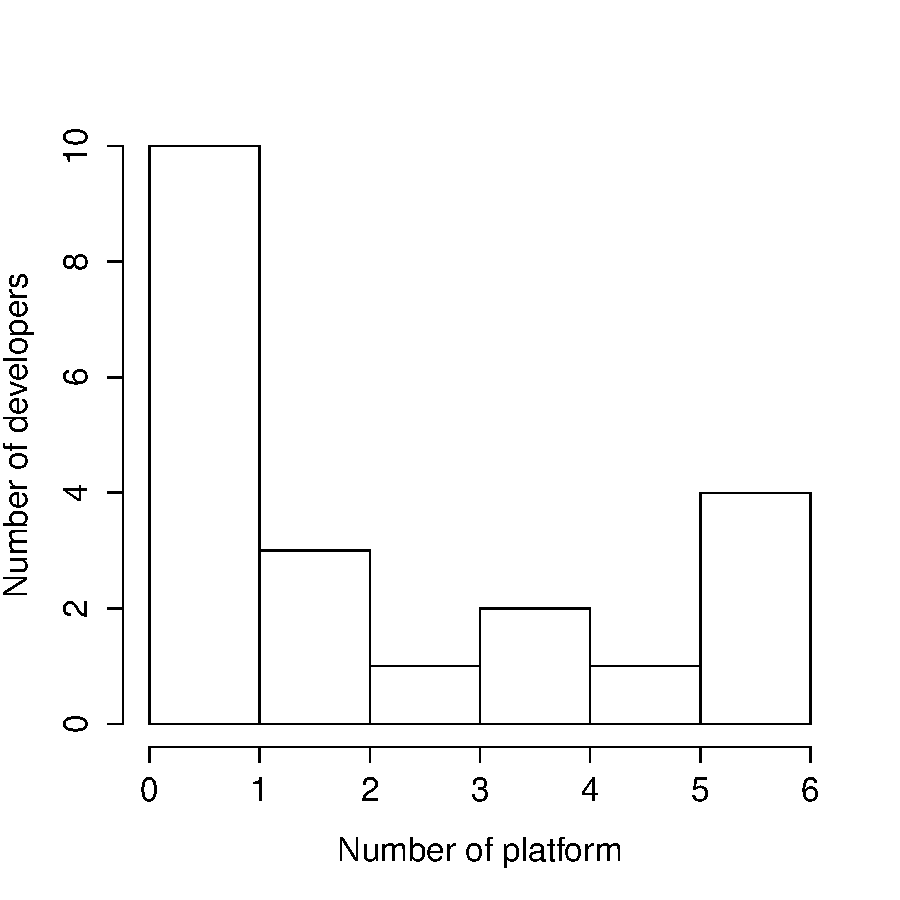
\includegraphics[width=2.5in]{DeveloperSpecialization}
\caption{Developer specialization}
\label{DeveloperSpecialization}
\end{figure}

Dividing the developers in core and peripheral team, we set the core team with 4 developers and the peripheral team with 17 developers. The core team was responsible for 97.7\% of the total number of commits. 

%\begin{table}[h]
%\renewcommand{\arraystretch}{1.3}
%\caption{Developer grouping}
%\label{devgrouping}
%\centering
%\begin{tabular}{|c|c|c|}
%\hline
%  & Team size   & Commits (\%) \\
%\hline
%Core & 4& 97.7 \\
%\hline
%Peripheral & 17 & 2.2\\
%\hline
%\end{tabular}
%\end{table} 

Our investigation shows that all core developers work with all six platforms and that peripheral developers tend to be specialized in a single platform, as 47.7\% of them work with one platform only. We also found that 11.17\% of peripheral developers support just the platform-independent code. The Table \ref{plat} presents all information about the number of platform core and peripheral developer support.    

%\todo[inline]{Eh a primeira vez que voce fala sobre platform-independent code; isso nao foi explicado antes.}

\begin{table}[h]
\renewcommand{\arraystretch}{1.3}
\caption{Number of platform core and peripheral developer support}
\label{plat}
\centering
\begin{tabular}{|c|c|c|c|}
\hline
Number of  & Core  & Peripheral  & All developers\\
	platform		& (\%)		&   (\%) 	&	(\%)	\\				
\hline
0 &   - &   11.17	& 9.5\\
\hline
1 &   - &   47.7	& 38.1\\
\hline
2 &   -&    17.7	&	14.3\\
\hline
3 &   - &   5.5	&	4.8\\
\hline
4 &   - &   11.1	&	9.5\\
\hline
5 &   - &   5.5 	& 4.8\\
\hline
6 &   100 &   -  	&	19.0\\
\hline
\end{tabular}
\end{table} 






%%%%%%%%%%%%%%%%%%%%%%%%%%%%%%%%%
\subsection{Results: Is there a clear separation between mobile and desktop developers?}

%\todo[inline]{Change the analysis... consider all developers first}
%As Allegro support different device types, we investigated in RQ2 if there was a separation in the developer team according to the device type. The results considering all developers groups together show that 23.31\% of the developers support desktop devices only, 14.49\% support mobile devices only and 52.28\% support both device types. As about half of the developers support both device types, we consider that there is no clear separation between mobile and desktop developers. Moreover, all core developers support both device types, that means that none of them are responsible for the code of a device type.
The Table \ref{devicetype} shows the device type specialization of the  developers. We measured the platform specialization for all developers and also for core and peripheral developer groups. Considering all developers, the results show that 52.28\%  of the developers support both device types, 23.31\% of the developers support desktop devices only and 14.49\% support mobile devices only.

In the core team, all developers support both device types. But in peripheral team, just 41.18\% of the developers support desktop and mobile platforms.       

%\todo[inline]{O caption da Tabela VI deveria permitir ao leitor entender a tabela sem ler o texto fora da tabela. Em particular, deveria explicar o que sao as porcentagens.}

\begin{table}[h]
\renewcommand{\arraystretch}{1.3}
\caption{Device type specialization of developers}
\label{devicetype}
\centering
\begin{tabular}{|c|c|c|c|}
\hline
 Device type & Core   & Peripheral &All developers \\
  &  (\%)   &  (\%) &  (\%)\\
\hline
Independent code only &     - &     11.1  &   9.92\\
\hline
Desktop only &          - &     29.9  &   23.31\\
\hline
Mobile only &           - &     17.7  &   14.49\\
\hline
Desktop and Mobile &      100 &     41.18 &   52.28 \\
\hline

\end{tabular}
\end{table} 




%%%%%%%%%%%%%%%%%%%%%%%%%%%%%%%%
\subsection{Results: Which platforms are more related together considering the set of platforms a developer work with? }

%We verified how many packages are touched in a commit for each platform, the results are shown in Figure \ref{packagesbyplatform}. The Figure \ref{packagesbyplatform} can be interpreted as: when a platform package is touched in a maintenance task, how many packages are also modified? Except Unix that have the median equals to two, all other five platforms have the minimum and median equals to 1, with special attention to macOS that also have third quartile equal to 1.  

%\todo[inline]{1 nao eh o maximo do macOS, eh o seu terceiro quartil.}
%\todo[inline]{Mais uma vez aparece o numero de pacotes em uma analise, resquicio de analises anteriores, mas que nao cabe na proposta deste artigo. Se fosse plataforma vs plataforma, melhor.}

%\begin{figure}[h]
%\centering
%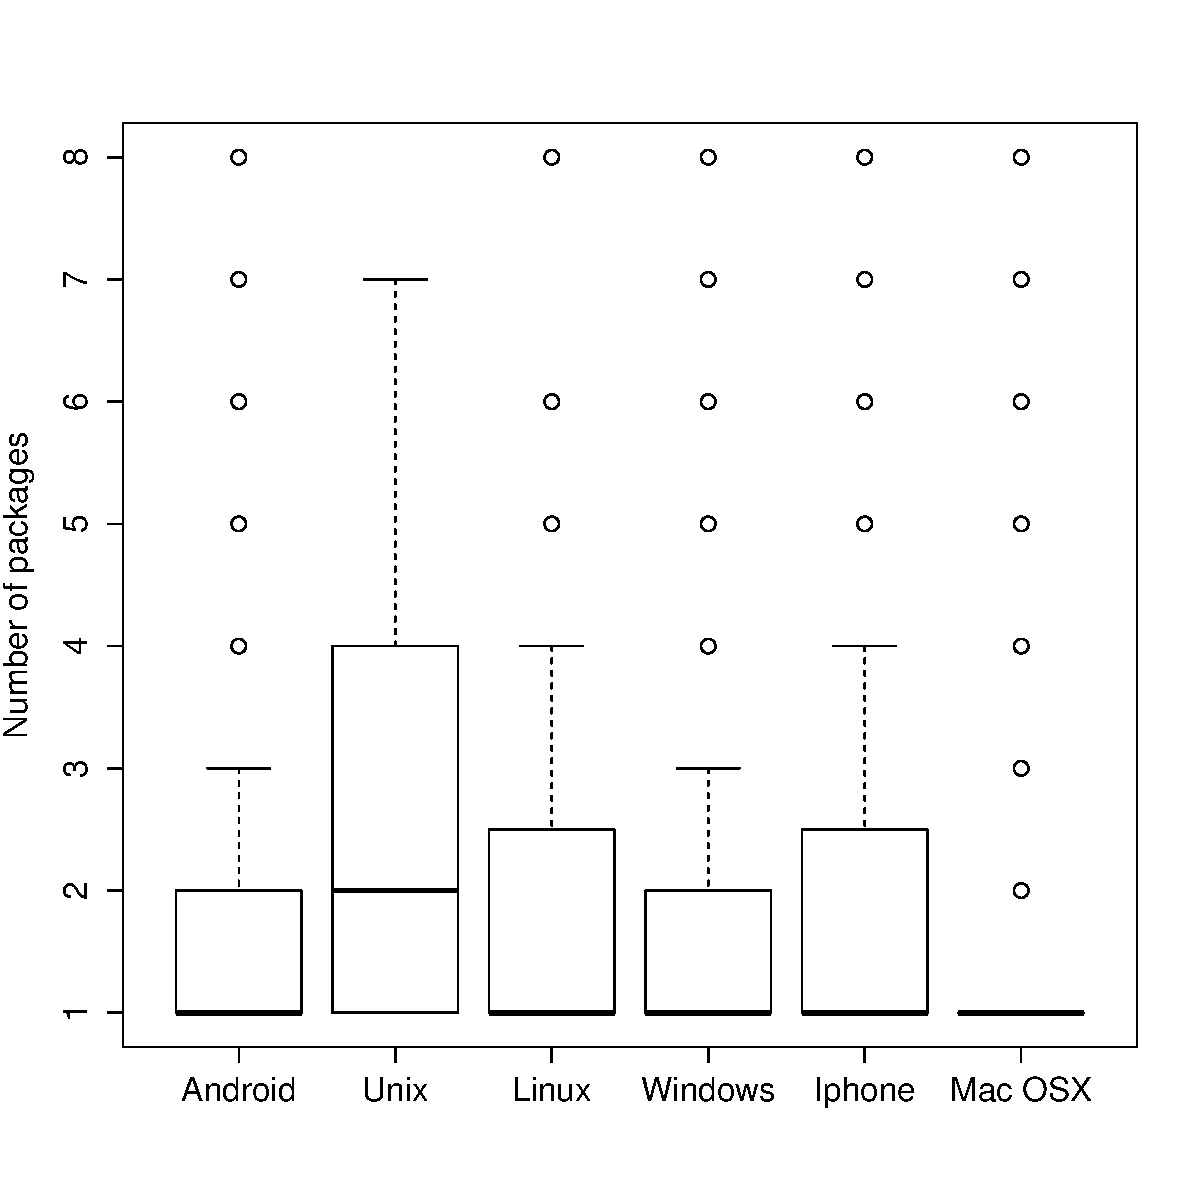
\includegraphics[width=3.0in]{packagesbyplatform}
%\caption{Number of packages touched in a commit for each platform}
%\label{packagesbyplatform}
%\end{figure}

The Apriori association rule results can be seen in Table \ref{assocrule}. The data set used in the association analysis was the set of platforms each developer works with, and each set of platforms is referred as a transaction. We analyzed 21 transactions with Apriori algorithm. 

All five association rules found relate desktop with mobile platforms. The association rule 1 shows that even though iPhone and Windows platform are from different device types and their are not logically coupled, as we can see in Figure \ref{allegroinfo}, developers who work with iPhone also work with Windows with a support of 0,38 and confidence of 0.89. 

Similar cases happened to the other rules. The rule 2, 3 and 4 was found in 7 out of 21  transactions with a confidence of 1.00.  The rule 5 was found in 7 out of 21 transactions with a confidence of 0.88. 

%\todo[inline]{Transactions sao um termo de association rule? Melhor falar de commits.}

%\todo[inline]{Quando voce diz out of 21, voce nao quer dizer que o total sao 21 commits, certo?}




\begin{table}[h]
\renewcommand{\arraystretch}{1.3}
\caption{Apriori association rule}
\label{assocrule}
\centering
\begin{tabular}{|c|c c c|c|c|}
\hline
 \# & \multicolumn{3}{|c|}{Association rule} & Supp. & Conf. \\
\hline
1&  \{iPhone\}      &$\Rightarrow$  &   \{Windows\} &   0.38  &   0.89  \\
\hline
2&  \{Linux\}       & $\Rightarrow$ &   \{Android\} &   0.33  &   1.00  \\
\hline
3&  \{iPhone, macOS\} &$\Rightarrow$  &   \{Windows\} &   0.33  &   1.00  \\
\hline
4&  \{Windows, macOS\} &$\Rightarrow$&    \{iPhone\}  &   0.33  &   1.00  \\
\hline
5&  \{Windows, iPhone\} &$\Rightarrow$&    \{macOS\}  &   0.33  &   0.88  \\
\hline
\end{tabular}
\end{table} 

%\todo[inline]{Vale a pena comentar que essa associacao entre iPhone e Windows eh contra-intuitiva.}
%2222

\section{Threats to validity}

%\todo[inline]{Acho que vale a pena mencionar brevemente as ameacas aa validade aqui na conclusao.}

Some threats to validity were identified in this research and we present them  following the usual category threats: internal, external, construct and conclusion validity.

%\todo[inline]{History: the circumstances are not the same on both occasions}
%\todo[inline]{Maturation: subjects react differently as time passes}
\begin{enumerate}

\item Internal validity: Allegro started supporting Windows, macOS and Linux from the very beginning of the project, iPhone in October 2009 and Android in December 2011. Hence, the platform-specific codes have different maturities and may demand different maintenance tasks. Another risk is that we did not consider the developer experience time in the analysis.  
%Interaction  of  selection  and  treatment.

%\todo[inline]{Interaction  of  selection  and  treatment}
\item External validity: the results obtained with Allegro cannot be generalized to other cross-platform libraries. However, this study can be replied using other cross-platform libraries.

%\todo[inline]{Inadequate preoperational explication of constructs or hypothesis guessing}
\item Construct validity: the lack of documentation of Allegro about the development process and how platform packages communicate can put at risk the study as we relied on metric measures to understand the package coupling and the developer team were divided in core and peripheral following recommendations from other researchers. 

%\todo[inline]{Reliability of measures}
\item Conclusion validity: for determining the set of platforms a developer support, we considered that if a developer touched a platform package in a commit, the developer support this platform. But we did not verified  what was the modification and the developer could have only added a comment in a file, for example. Another threat is that the developers can support more platforms than the ones we considered because Allegro support other platforms unofficially. 

\end{enumerate}





%%%%%%%%%%%%%%%%%%%%%%%%%%%%%%%%%%%%%%
%%%%%%%%%%%%%%%%%%%%%%%%%%%%%%%%%%%%%%
%%%%%%%%%%%%%%%%%%%%%%%%%%%%%%%%%%%%%%
\section{Conclusion}
\label{conclusion}

The development of cross-platform libraries can alleviate the developer work load in building cross-platform applications and promotes software reuse. Details of implementation of cross-platform libraries are still unknown and there is no worldwide method for building software for multiple platforms. %Details of implementation of cross-platform libraries are not well defined and many developers use such libraries as a black box.  

%Do core developers tend to contribute with more platforms than peripheral developers?
Allegro's core developers support all six platforms analyzed, while only 40\% of the peripheral developers support more than one platform. Therefore, answering the RQ1, we conclude that the core developers support more platforms than peripheral developers. The results also prove that the Allegro's core developer team is highly qualified, as they support all six platforms. 

%Is there a clear separation between mobile and desktop developers?
As Allegro support different device types, we investigated in RQ2 if there was a separation in the developer team according to the device type. The results considering all developers groups together show that 23.31\% of the developers support desktop devices only, 14.49\% support mobile devices only and 52.28\% support both device types. As about half of the developers support both device types, we consider that there is no clear separation between mobile and desktop developers. Moreover, all core developers support both device types, that means that none of them are responsible for the code of a device type.  

%Which platforms are more related together considering the set of platforms a developer work with? 
In the association analysis we performed to identify relationships among platforms a developer work with, we found five rules relating platforms of different device types. The rule 1 happened to be true in 38\% of the transactions and rule 2, 3, 4 and 5 happen to be true in 33\% of the transactions.  Actually this fact was not expected but despite of that we found strong relationships among some platforms, listed in Table \ref{assocrule}. 

Still there is a lot to investigate about cross-platform libraries. We plan to replicate this study using other cross-platform libraries and we also want to expand on this research by investigating other subjects:
\begin{itemize}
 
\item Platform-specific and independent code: verify if developers mix the platform-specific and independent code in the same file checking conditional compilation flags within a file.

\item Modularity: use co-changes to assess the modularity of cross-platform libraries. 

\item Platform support: chronologically, study the gap between the appearance of a platform and its support by a cross-platform library.

\end{itemize}



%\cite{Robles2009} % Core peripheral developer
%\cite{backblaze2008} % ten rules
%\cite{Levin2014} %Book
%\cite{Duc2014} ¨% Forking and Coordination
%\cite{Tan2005}% Introduction to data mining book
%\cite{bishop2006} % software that lasts
%\cite{Fahy2012} %Using open source libraries in cross platform games development


%\cite{Nebeling2013} % Informing the Design of New Mobile Development Methods and Tools
%\cite{Sorensen2014} % The 4C Framework: Principles of Interaction in Digital Ecosystems
%\cite{Dong2016} %Understanding the Challenges of Designing and Developing Multi-Device Experiences
%\cite{Catalyst} %Bermuda triangle

% conference papers do not normally have an appendix


% use section* for acknowledgement

%\section*{Acknowledgment}
%The authors would like to thank...
%more thanks here


% trigger a \newpage just before the given reference
% number - used to balance the columns on the last page
% adjust value as needed - may need to be readjusted if
% the document is modified later
%\IEEEtriggeratref{8}
% The "triggered" command can be changed if desired:
%\IEEEtriggercmd{\enlargethispage{-5in}}

% references section

% can use a bibliography generated by BibTeX as a .bbl file
% BibTeX documentation can be easily obtained at:
% http://www.ctan.org/tex-archive/biblio/bibtex/contrib/doc/
% The IEEEtran BibTeX style support page is at:
% http://www.michaelshell.org/tex/ieeetran/bibtex/
\bibliographystyle{IEEEtran}
% argument is your BibTeX string definitions and bibliography database(s)
\bibliography{bib}
%
% <OR> manually copy in the resultant .bbl file
% set second argument of \begin to the number of references
% (used to reserve space for the reference number labels box)
%\begin{thebibliography}{1}



%\bibitem{IEEEhowto:kopka}
%H.~Kopka and P.~W. Daly, \emph{A Guide to \LaTeX}, 3rd~ed.\hskip 1em plus
 % 0.5em minus 0.4em\relax Harlow, England: Addison-Wesley, 1999.

%\end{thebibliography}




% that's all folks
\end{document}


